
\subsection{Depth Estimation}
We evaluate the depth estimation models described in \cref{sec:stereo_depth_estimation,sec:monocular_depth_estimation} in the LuSNAR dataset.
\Cref{fig:depth_errors} shows the RGB input and the depth errors for different depth estimation models in logarithmic scale to qualitatively characterize the performance of the models.
Traditional stereo methods like BM and SGBM perform well under favorable illumination conditions but struggle when the light source is behind the camera or when dealing with bright areas and shadows. Learning-based stereo models, particularly RAFT-Stereo, demonstrate superior performance with high depth completion rates and excellent accuracy at short distances. While monocular models lag behind even after proper scaling, achieving error rates comparable to previous models only at medium distances, they could still be valuable for surface reconstruction when combined with proper uncertainty quantification, as they provide significantly more information than RGB images alone.


\Cref{tab:depth_models} shows the quantitative results of the depth estimation models.
Traditional stereo methods achieve low MAE and AbsRel by producing depth only in regions where they are confident, which is evident from their low $\delta_{25\%}$ values. Learning-based stereo models like RAFT-Stereo predict depth more densely, including at longer ranges, which increases MAE due to larger absolute errors at far distances. However, the AbsRel remains comparable, indicating that relative errors remain low across distances. These models also operate at significantly lower frame rates compared to traditional methods. Monocular models underperform across all metrics, even after scale correction, but remain potentially useful when stereo input is not available. Since they are trained on Earth-based datasets, their performance on this terrain requires further evaluation, particularly with respect to finetuning.
\begin{table}[t]
	\centering
	\small
	\caption{\bfseries Comparison of depth estimation models. Monocular depth is scaled using triangulated points from matched features.}
	\label{tab:depth_models}
	\begin{tabular}{|lrrrrr|}
		\hline
		\textbf{Model}                          &
		\textbf{Params}                         &
		\textbf{MAE}$\downarrow$                &
		\textbf{AbsRel}$\downarrow$             &
		\textbf{$\delta_{25\%}$}$\uparrow$      &
		\textbf{FPS}$\uparrow$                                                     \\
		\hline\hline
		\textbf{Stereo}                         &      &      &      &      &      \\
		BM                                      & --   & 1.6  & 0.02 & 0.30 & 24.5 \\
		SGBM                                    & --   & 1.6  & 0.02 & 0.41 & 14.9 \\
		RAFT-Stereo                             & 11M  & 7.3  & 0.05 & 0.72 & 4.5  \\
		CREStereo                               & 5M   & 3.5  & 0.04 & 0.73 & 1.4  \\
		\hline\hline
		\multicolumn{2}{|l}{\textbf{Monocular}} &      &      &      &             \\
		\multicolumn{2}{|l}{Depth Anything V2}  &      &      &      &             \\
		~ Small                                 & 25M  & 11.1 & 0.21 & 0.53 & 13.2 \\
		~ Base                                  & 97M  & 10.8 & 0.19 & 0.56 & 13.2 \\
		~ Large                                 & 335M & 10.7 & 0.18 & 0.59 & 9.8  \\
		GLPN                                    & 61M  & 15.1 & 1.82 & 0.07 & 9.9  \\
		DPT                                     & 343M & 11.2 & 0.19 & 0.55 & 13.6 \\
		Depth Pro                               & 952M & 11.4 & 0.20 & 0.55 & 1.7  \\
		\hline
	\end{tabular}
\end{table}

\cref{fig:depth_stereo_lusnar} shows the performance of RAFT-Stereo. The model shows consistent performance with high accuracy in near regions (below 5 cm error). Precise depth estimates even in challenging lighting conditions and complex geometries.
\begin{figure}[h]
	\centering
	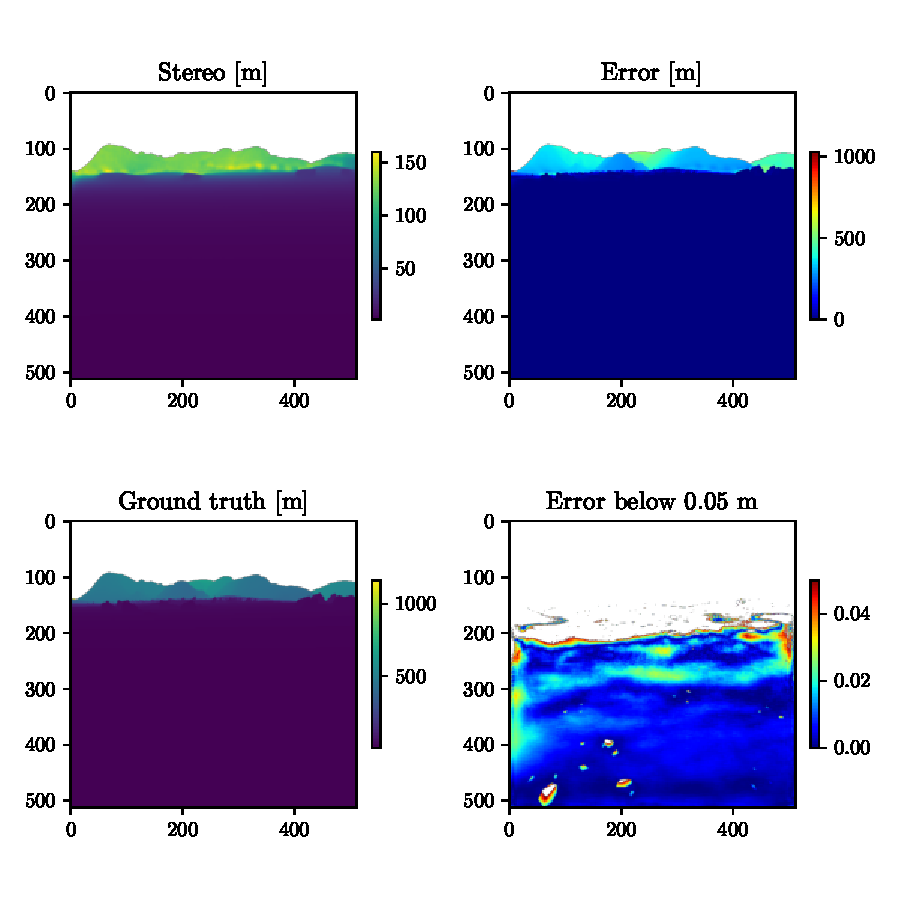
\includegraphics[width=\linewidth]{figures/depth_stereo_lusnar.pdf}
	\caption{\bfseries LuSNAR dataset.}
	\label{fig:depth_stereo_lusnar}
\end{figure}